
%% bare_conf.tex
%% V1.4b
%% 2015/08/26
%% by Michael Shell
%% See:
%% http://www.michaelshell.org/
%% for current contact information.
%%
%% This is a skeleton file demonstrating the use of IEEEtran.cls
%% (requires IEEEtran.cls version 1.8b or later) with an IEEE
%% conference paper.
%%
%% Support sites:
%% http://www.michaelshell.org/tex/ieeetran/
%% http://www.ctan.org/pkg/ieeetran
%% and
%% http://www.ieee.org/

%%*************************************************************************
%% Legal Notice:
%% This code is offered as-is without any warranty either expressed or
%% implied; without even the implied warranty of MERCHANTABILITY or
%% FITNESS FOR A PARTICULAR PURPOSE! 
%% User assumes all risk.
%% In no event shall the IEEE or any contributor to this code be liable for
%% any damages or losses, including, but not limited to, incidental,
%% consequential, or any other damages, resulting from the use or misuse
%% of any information contained here.
%%
%% All comments are the opinions of their respective authors and are not
%% necessarily endorsed by the IEEE.
%%
%% This work is distributed under the LaTeX Project Public License (LPPL)
%% ( http://www.latex-project.org/ ) version 1.3, and may be freely used,
%% distributed and modified. A copy of the LPPL, version 1.3, is included
%% in the base LaTeX documentation of all distributions of LaTeX released
%% 2003/12/01 or later.
%% Retain all contribution notices and credits.
%% ** Modified files should be clearly indicated as such, including  **
%% ** renaming them and changing author support contact information. **
%%*************************************************************************


% *** Authors should verify (and, if needed, correct) their LaTeX system  ***
% *** with the testflow diagnostic prior to trusting their LaTeX platform ***
% *** with production work. The IEEE's font choices and paper sizes can   ***
% *** trigger bugs that do not appear when using other class files.       ***                          ***
% The testflow support page is at:
% http://www.michaelshell.org/tex/testflow/



\documentclass[conference]{IEEEtran}
\usepackage[utf8]{inputenc}
\usepackage[T1]{fontenc}
% Some Computer Society conferences also require the compsoc mode option,
% but others use the standard conference format.
%
% If IEEEtran.cls has not been installed into the LaTeX system files,
% manually specify the path to it like:
% \documentclass[conference]{../sty/IEEEtran}





% Some very useful LaTeX packages include:
% (uncomment the ones you want to load)


% *** MISC UTILITY PACKAGES ***
%
%\usepackage{ifpdf}
% Heiko Oberdiek's ifpdf.sty is very useful if you need conditional
% compilation based on whether the output is pdf or dvi.
% usage:
% \ifpdf
%   % pdf code
% \else
%   % dvi code
% \fi
% The latest version of ifpdf.sty can be obtained from:
% http://www.ctan.org/pkg/ifpdf
% Also, note that IEEEtran.cls V1.7 and later provides a builtin
% \ifCLASSINFOpdf conditional that works the same way.
% When switching from latex to pdflatex and vice-versa, the compiler may
% have to be run twice to clear warning/error messages.






% *** CITATION PACKAGES ***

\usepackage{cite}
% cite.sty was written by Donald Arseneau
% V1.6 and later of IEEEtran pre-defines the format of the cite.sty package
% \cite{} output to follow that of the IEEE. Loading the cite package will
% result in citation numbers being automatically sorted and properly
% "compressed/ranged". e.g., [1], [9], [2], [7], [5], [6] without using
% cite.sty will become [1], [2], [5]--[7], [9] using cite.sty. cite.sty's
% \cite will automatically add leading space, if needed. Use cite.sty's
% noadjust option (cite.sty V3.8 and later) if you want to turn this off
% such as if a citation ever needs to be enclosed in parenthesis.
% cite.sty is already installed on most LaTeX systems. Be sure and use
% version 5.0 (2009-03-20) and later if using hyperref.sty.
% The latest version can be obtained at:
% http://www.ctan.org/pkg/cite
% The documentation is contained in the cite.sty file itself.






% *** GRAPHICS RELATED PACKAGES ***
%
\ifCLASSINFOpdf
  % \usepackage[pdftex]{graphicx}
  % declare the path(s) where your graphic files are
  % \graphicspath{{../pdf/}{../jpeg/}}
  % and their extensions so you won't have to specify these with
  % every instance of \includegraphics
  % \DeclareGraphicsExtensions{.pdf,.jpeg,.png}
\else
  % or other class option (dvipsone, dvipdf, if not using dvips). graphicx
  % will default to the driver specified in the system graphics.cfg if no
  % driver is specified.
  % \usepackage[dvips]{graphicx}
  % declare the path(s) where your graphic files are
  % \graphicspath{{../eps/}}
  % and their extensions so you won't have to specify these with
  % every instance of \includegraphics
  % \DeclareGraphicsExtensions{.eps}
\fi
% graphicx was written by David Carlisle and Sebastian Rahtz. It is
% required if you want graphics, photos, etc. graphicx.sty is already
% installed on most LaTeX systems. The latest version and documentation
% can be obtained at: 
% http://www.ctan.org/pkg/graphicx
% Another good source of documentation is "Using Imported Graphics in
% LaTeX2e" by Keith Reckdahl which can be found at:
% http://www.ctan.org/pkg/epslatex
%
% latex, and pdflatex in dvi mode, support graphics in encapsulated
% postscript (.eps) format. pdflatex in pdf mode supports graphics
% in .pdf, .jpeg, .png and .mps (metapost) formats. Users should ensure
% that all non-photo figures use a vector format (.eps, .pdf, .mps) and
% not a bitmapped formats (.jpeg, .png). The IEEE frowns on bitmapped formats
% which can result in "jaggedy"/blurry rendering of lines and letters as
% well as large increases in file sizes.
%
% You can find documentation about the pdfTeX application at:
% http://www.tug.org/applications/pdftex





% *** MATH PACKAGES ***
%
%\usepackage{amsmath}
% A popular package from the American Mathematical Society that provides
% many useful and powerful commands for dealing with mathematics.
%
% Note that the amsmath package sets \interdisplaylinepenalty to 10000
% thus preventing page breaks from occurring within multiline equations. Use:
%\interdisplaylinepenalty=2500
% after loading amsmath to restore such page breaks as IEEEtran.cls normally
% does. amsmath.sty is already installed on most LaTeX systems. The latest
% version and documentation can be obtained at:
% http://www.ctan.org/pkg/amsmath





% *** SPECIALIZED LIST PACKAGES ***
%
%\usepackage{algorithmic}
% algorithmic.sty was written by Peter Williams and Rogerio Brito.
% This package provides an algorithmic environment fo describing algorithms.
% You can use the algorithmic environment in-text or within a figure
% environment to provide for a floating algorithm. Do NOT use the algorithm
% floating environment provided by algorithm.sty (by the same authors) or
% algorithm2e.sty (by Christophe Fiorio) as the IEEE does not use dedicated
% algorithm float types and packages that provide these will not provide
% correct IEEE style captions. The latest version and documentation of
% algorithmic.sty can be obtained at:
% http://www.ctan.org/pkg/algorithms
% Also of interest may be the (relatively newer and more customizable)
% algorithmicx.sty package by Szasz Janos:
% http://www.ctan.org/pkg/algorithmicx




% *** ALIGNMENT PACKAGES ***
%
%\usepackage{array}
% Frank Mittelbach's and David Carlisle's array.sty patches and improves
% the standard LaTeX2e array and tabular environments to provide better
% appearance and additional user controls. As the default LaTeX2e table
% generation code is lacking to the point of almost being broken with
% respect to the quality of the end results, all users are strongly
% advised to use an enhanced (at the very least that provided by array.sty)
% set of table tools. array.sty is already installed on most systems. The
% latest version and documentation can be obtained at:
% http://www.ctan.org/pkg/array


% IEEEtran contains the IEEEeqnarray family of commands that can be used to
% generate multiline equations as well as matrices, tables, etc., of high
% quality.




% *** SUBFIGURE PACKAGES ***
%\ifCLASSOPTIONcompsoc
%  \usepackage[caption=false,font=normalsize,labelfont=sf,textfont=sf]{subfig}
%\else
%  \usepackage[caption=false,font=footnotesize]{subfig}
%\fi
% subfig.sty, written by Steven Douglas Cochran, is the modern replacement
% for subfigure.sty, the latter of which is no longer maintained and is
% incompatible with some LaTeX packages including fixltx2e. However,
% subfig.sty requires and automatically loads Axel Sommerfeldt's caption.sty
% which will override IEEEtran.cls' handling of captions and this will result
% in non-IEEE style figure/table captions. To prevent this problem, be sure
% and invoke subfig.sty's "caption=false" package option (available since
% subfig.sty version 1.3, 2005/06/28) as this is will preserve IEEEtran.cls
% handling of captions.
% Note that the Computer Society format requires a larger sans serif font
% than the serif footnote size font used in traditional IEEE formatting
% and thus the need to invoke different subfig.sty package options depending
% on whether compsoc mode has been enabled.
%
% The latest version and documentation of subfig.sty can be obtained at:
% http://www.ctan.org/pkg/subfig




% *** FLOAT PACKAGES ***
%
%\usepackage{fixltx2e}
% fixltx2e, the successor to the earlier fix2col.sty, was written by
% Frank Mittelbach and David Carlisle. This package corrects a few problems
% in the LaTeX2e kernel, the most notable of which is that in current
% LaTeX2e releases, the ordering of single and double column floats is not
% guaranteed to be preserved. Thus, an unpatched LaTeX2e can allow a
% single column figure to be placed prior to an earlier double column
% figure.
% Be aware that LaTeX2e kernels dated 2015 and later have fixltx2e.sty's
% corrections already built into the system in which case a warning will
% be issued if an attempt is made to load fixltx2e.sty as it is no longer
% needed.
% The latest version and documentation can be found at:
% http://www.ctan.org/pkg/fixltx2e


%\usepackage{stfloats}
% stfloats.sty was written by Sigitas Tolusis. This package gives LaTeX2e
% the ability to do double column floats at the bottom of the page as well
% as the top. (e.g., "\begin{figure*}[!b]" is not normally possible in
% LaTeX2e). It also provides a command:
%\fnbelowfloat
% to enable the placement of footnotes below bottom floats (the standard
% LaTeX2e kernel puts them above bottom floats). This is an invasive package
% which rewrites many portions of the LaTeX2e float routines. It may not work
% with other packages that modify the LaTeX2e float routines. The latest
% version and documentation can be obtained at:
% http://www.ctan.org/pkg/stfloats
% Do not use the stfloats baselinefloat ability as the IEEE does not allow
% \baselineskip to stretch. Authors submitting work to the IEEE should note
% that the IEEE rarely uses double column equations and that authors should try
% to avoid such use. Do not be tempted to use the cuted.sty or midfloat.sty
% packages (also by Sigitas Tolusis) as the IEEE does not format its papers in
% such ways.
% Do not attempt to use stfloats with fixltx2e as they are incompatible.
% Instead, use Morten Hogholm'a dblfloatfix which combines the features
% of both fixltx2e and stfloats:
%
% \usepackage{dblfloatfix}
% The latest version can be found at:
% http://www.ctan.org/pkg/dblfloatfix




% *** PDF, URL AND HYPERLINK PACKAGES ***
%
%\usepackage{url}
% url.sty was written by Donald Arseneau. It provides better support for
% handling and breaking URLs. url.sty is already installed on most LaTeX
% systems. The latest version and documentation can be obtained at:
% http://www.ctan.org/pkg/url
% Basically, \url{my_url_here}.




% *** Do not adjust lengths that control margins, column widths, etc. ***
% *** Do not use packages that alter fonts (such as pslatex).         ***
% There should be no need to do such things with IEEEtran.cls V1.6 and later.
% (Unless specifically asked to do so by the journal or conference you plan
% to submit to, of course. )


% correct bad hyphenation here
\hyphenation{op-tical net-works semi-conduc-tor}


\begin{document}
%
% paper title
% Titles are generally capitalized except for words such as a, an, and, as,
% at, but, by, for, in, nor, of, on, or, the, to and up, which are usually
% not capitalized unless they are the first or last word of the title.
% Linebreaks \\ can be used within to get better formatting as desired.
% Do not put math or special symbols in the title.
\title{
%Performance Factors for Large Scale Machine Learning Applications
A Beginners Guide to Perfomance Factors of Machine Learning Learning Applications with Focus on Neural Nets and Deep Learning
}

\author{\IEEEauthorblockN{Johannes Wünsche}
\IEEEauthorblockA{Otto-von-Guericke University Magdeburg\\
Email: johannes.wuensche@st.ovgu.de}
}

% make the title area
\maketitle

% As a general rule, do not put math, special symbols or citations
% in the abstract
\begin{abstract}
%\begin{itemize}
%\item Deliver short introduction for neural networks with different aspect focused examples
%\item What we want to show in this paper(performance factors)
%\item To what end we came
%\item some other stuff that comes up during the paper and is important enough to be named at the beginning
%\end{itemize}

Machine Learning is probably the most present topic of computer science in the media. This popularity only increased over the recent years thorugh widely publicly known apllications ranging from DeepBlue(not so recent) to IBM Watson and AlphaGo. Because of these successes Machine Learning is sometimes viewed as omnipotent solution to every imaginable problem. This is most certainly not the case, Neural Nets and alike are powerful but require a large amount of maintenance

\end{abstract}

\IEEEpeerreviewmaketitle
\section{Introduction}
Machine Learning seems to be everywhere around us. With the recent success of Deep, Convolutional,and Neural Networks, and other Machine Learning tools, especially the, in general media, well reported Learners like AlphaGo, Silver or Watson, these are experiencing a kind of renaissance their usage has spread from industrial(e.g. Self-driving cars rely on autonomous interpretation of camera feed and sensor output that can be optimized by using machine learning) to retail. But also in modern automation and research, machine learning becomes a greater field managing to find more efficient ways to achieve better results in many expertise.

In this paper we want to observe and identify the most performance influencing factors of theses networks while designing and implementing them for specific applications for both small and large scales.
We expect that this study will provide help for readers interested in learning about the requirements for managing data and operations of an efficient neural network.

TODO: related surveys

 At first we attend the choice of neural network and the impact of this decision. Afterwards we chose to have a look, on one hand, at small scale neural networks running on a single machine without large data sets and a low query frequency after the initial training, and at the other hand, large scale neural networks operating with more layers and nodes, large data sets and distributed system to handle the computational power required by the neural network training algorithms to be completed in reasonable time.

\section{Background}
The reader is advised to be familiar with the base idea of a neural network and some common types of networks like the deep, convolutional, feed forward and recurrent networks.

The most common neural network frameworks which we, because of their wide popularity, will mostly view are Tensorflow\cite{abadi2016tensorflow}, Caffe\cite{jia2014caffe}, Torch\cite{collobert2002torch}, CNTK, deeplearning4j, Keras, MXNET. These frameworks have been benchmarked in numerous settings and applications and can help us show performance influencing factors.


\section{Choice of Neural Nets}
what net when to use, and starting values of neural nets like amount of layers and starting weights

\section{Choice of Processing Unit}
The next important choice is the choice of the actual operating calculation unit. We distinguish them into three main models, CPU, GPU and GPU-Clustering.
\subsection{CPU}
As the first most naive option we looked on the CPU for training of the neural net with the simple single thread and more complex multi-thread calculation.
\subsubsection{Single-thread}
The most naive implementation is the single-thread CPU calculation, because oft this more  brute force approach and sequential execution and calculation this is also the slowest and with a larger number of connected nodes simply unfeasible because of the excessive calculation time required . But as can be thought of this does not uitilize the full capacity of the CPU and therefore results in performance loss in comparison to multithread usage(Fig. 1).
\subsubsection{Multi-thread}
A more complex approach consist of utilizing the multi-core characterisitics of modern CPUs, by splitting of training calculation with only requirements to already calculated values. This is for example preferrable when training with the help of a \emph{Backpropagation} algorithm. The effect  continues to grow by using more threads but reaches it limits when using more threads than physical cores available.
\begin{figure} 
\centering
\begin{tabular}{c c c c c}
\hline
Framework & 1 Thread & 2 Threads &4 Threads & 8 Threads\\\hline
Caffe & 1.324 & 0.790 & 0.578 & 15.444 \\
Tensorflow & 7.062 & 4.789 & 2.648 & 1.938 \\
Torch & 1.329 & 0.710 & 0.423 & na \\\hline
\end{tabular}
\caption{Training time(in s) for a mini-batch of size 64 of a Fully Connected Network(FCN) trained with synthetic data on a i7-3820 with 4-physical cores using 3 different commonly used Deep Learning frameworks\cite{shi2016benchmarking}}
\label{fig_ttfcn}
\end{figure}

Though this approach is limited by the actual core number available and should not overstep the number of physical cores, like with intel \emph{hyper-threading} technology, which can lengthen the required calculation time because of a more inefficient usage\cite{shi2016benchmarking}.
\subsection{GPU}
A more advanced implementation is to use the shared memory, multi-core environment of modern GPUs. For example with NVIDIAs CUDA this can be done efficiently and result in a speed-up of calculation of up to 3 times the CPU-based approachs performance for deep learning algorithms over optimized floting-point baseline\cite{shi2016benchmarking}. Allmost all recent neural net learning frameworks support this calculation unit because of its excellent performance rating for neural networks.

Problems lie in the tightly restricted memory of graphic cards that may not be able to contain all nodes with their corresponding weights as well as training dataset. This leads to some communication overhead depending on the communication strategy chosen.

%\begin{figure}
%\centering
%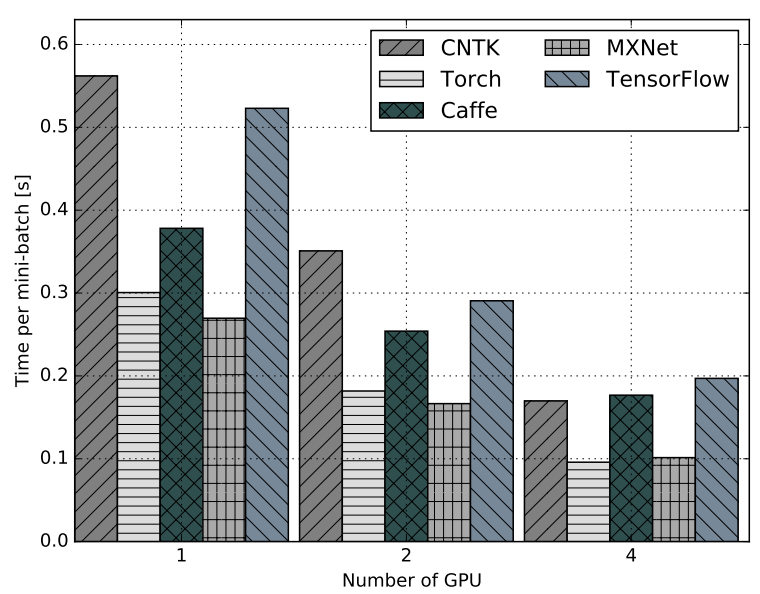
\includegraphics[width=0.2\textwidth]{a.png}
%
%\caption{Time per mini-batch in s compared between different amount of GPUs used\cite{shi2016benchmarking}}
%\label{fig_m_gpu}
%\end{figure}


\subsection{GPU-Cluster}
The next logical step is to use multiple GPUs further reducing training time but also creating new challenges, because of the decentralized nature of the Cluster, like communication overhead.  This is mostly used in large scale applications and is most of the time not needed in small scale.

A main advantage of the Cluster is of course the increased computation power available during the training phase, reducing training time by 35\% when doubling the number of GPUs in CNTK and MXNET, 28 \% in Caffe and 10 \% in  Torch and Tensorflow\cite{shi2016benchmarking}.

Another advantage is the greater availability of memory somewhat easing the restrictions of the memory restricted GPUs structure. While this is an advantage it is not efficient if used as the single goal of multiple GPU usage because of the high price connected to acquiring them.

Fig. 2 visualizes this improvement showing the reduction of training time steadily with the increasing of amount of GPUs used. Although costly this leads to a constant improvement. Higher Numbers of GPUs can be again slower or offer no significant improvement if used the same as smaller amounts because of an increasing communication overhead and bottleneck in the CPU, which is responsible for managing seperate GPUs.

\subsubsection{Multiple GPU-Clusters}
Taking a step further it is possible to connect multiple Clusters of GPUs to compute a single task. In doing this we again increase raw computation power, but also increase the total amount of communication required.

\section{Scaling challenges}
Here I want to clarify a bit on strategies to create an efficient CPU-GPUs interchange with as little overhead as possible.
TODO: Spanish thesis on SuperComputer Learning

% An example of a floating figure using the graphicx package.
% Note that \label must occur AFTER (or within) \caption.
% For figures, \caption should occur after the \includegraphics.
% Note that IEEEtran v1.7 and later has special internal code that
% is designed to preserve the operation of \label within \caption
% even when the captionsoff option is in effect. However, because
% of issues like this, it may be the safest practice to put all your
% \label just after \caption rather than within \caption{}.
%
% Reminder: the "draftcls" or "draftclsnofoot", not "draft", class
% option should be used if it is desired that the figures are to be
% displayed while in draft mode.
%
%\begin{figure}[!t]
%\centering
%\includegraphics[width=2.5in]{myfigure}
% where an .eps filename suffix will be assumed under latex, 
% and a .pdf suffix will be assumed for pdflatex; or what has been declared
% via \DeclareGraphicsExtensions.
%\caption{Simulation results for the network.}
%\label{fig_sim}
%\end{figure}

% Note that the IEEE typically puts floats only at the top, even when this
% results in a large percentage of a column being occupied by floats.


% An example of a double column floating figure using two subfigures.
% (The subfig.sty package must be loaded for this to work.)
% The subfigure \label commands are set within each subfloat command,
% and the \label for the overall figure must come after \caption.
% \hfil is used as a separator to get equal spacing.
% Watch out that the combined width of all the subfigures on a 
% line do not exceed the text width or a line break will occur.
%
%\begin{figure*}[!t]
%\centering
%\subfloat[Case I]{\includegraphics[width=2.5in]{box}%
%\label{fig_first_case}}
%\hfil
%\subfloat[Case II]{\includegraphics[width=2.5in]{box}%
%\label{fig_second_case}}
%\caption{Simulation results for the network.}
%\label{fig_sim}
%\end{figure*}
%
% Note that often IEEE papers with subfigures do not employ subfigure
% captions (using the optional argument to \subfloat[]), but instead will
% reference/describe all of them (a), (b), etc., within the main caption.
% Be aware that for subfig.sty to generate the (a), (b), etc., subfigure
% labels, the optional argument to \subfloat must be present. If a
% subcaption is not desired, just leave its contents blank,
% e.g., \subfloat[].


% An example of a floating table. Note that, for IEEE style tables, the
% \caption command should come BEFORE the table and, given that table
% captions serve much like titles, are usually capitalized except for words
% such as a, an, and, as, at, but, by, for, in, nor, of, on, or, the, to
% and up, which are usually not capitalized unless they are the first or
% last word of the caption. Table text will default to \footnotesize as
% the IEEE normally uses this smaller font for tables.
% The \label must come after \caption as always.
%
%\begin{table}[!t]
%% increase table row spacing, adjust to taste
%\renewcommand{\arraystretch}{1.3}
% if using array.sty, it might be a good idea to tweak the value of
% \extrarowheight as needed to properly center the text within the cells
%\caption{An Example of a Table}
%\label{table_example}
%\centering
%% Some packages, such as MDW tools, offer better commands for making tables
%% than the plain LaTeX2e tabular which is used here.
%\begin{tabular}{|c||c|}
%\hline
%One & Two\\
%\hline
%Three & Four\\
%\hline
%\end{tabular}
%\end{table}


% Note that the IEEE does not put floats in the very first column
% - or typically anywhere on the first page for that matter. Also,
% in-text middle ("here") positioning is typically not used, but it
% is allowed and encouraged for Computer Society conferences (but
% not Computer Society journals). Most IEEE journals/conferences use
% top floats exclusively. 
% Note that, LaTeX2e, unlike IEEE journals/conferences, places
% footnotes above bottom floats. This can be corrected via the
% \fnbelowfloat command of the stfloats package.




\section{Conclusion}
yeah ... pretty much the conclusion shortly repeating the basis that is important for it and point the way they were created, should be larger part to emphasize the importance of some factors over others and the reasoning behind this classification
\cite{shi2016benchmarking}

TODO: Takeaway, different ideas, innnovative

% use section* for acknowledgment
\section*{Acknowledgment}
The author would like to thank Gabriel Campero Durand for advise and help to write the paper





% trigger a \newpage just before the given reference
% number - used to balance the columns on the last page
% adjust value as needed - may need to be readjusted if
% the document is modified later
%\IEEEtriggeratref{8}
% The "triggered" command can be changed if desired:
%\IEEEtriggercmd{\enlargethispage{-5in}}

\bibliographystyle{IEEEtran}
\bibliography{paper}


% that's all folks
\end{document}


